\documentclass[10pt,twocolumn]{jarticle}
\usepackage[dvipdfmx]{graphicx}
\graphicspath{ {EMG-images/} }
\usepackage{amsmath}
\usepackage{geometry}
\geometry{body={175mm,260mm},columnsep=8mm}

\title{表面筋電図計測}
\author{}
\date{}

\begin{document}
\maketitle
\section{筋電をとる前に}
\subsection{筋収縮のメカニズム}
筋活動は,脊髄のなかにある{\bf $\alpha$運動ニューロン}
  ($\alpha$-MotoNeuron : $\alpha$-MN)の興奮から始まり,その興奮インパ
ルスが{\bf 神経軸索}を経由して目指す筋に伝えられる.
\begin{figure}[b]
  \begin{center}
    \includegraphics[width=8cm,height=4cm,keepaspectratio,clip]{emg001.eps} 
    \label{fig:fig1}
    \includegraphics[width=8cm,height=5.3cm,keepaspectratio,clip]{emg002.eps} 
    \label{fig:fig2}
  \end{center}
\end{figure}
神経軸索は筋の中で枝わかれし,多数の{\bf 筋線維}(muscle fiber)に{\bf
  神経筋接合部}(neuromuscular junction)($=$神経終板(endplate))を作って
おり,1つの筋線維上には,通常1ヶ所の神経筋接合部が存在する.
1つの運動ニューロンに支配された筋線維群の活動は1つの単位として機能し,
それらをまとめて{\bf 運動単位}(Motor Unit : MU)と呼ぶ(図\ref{fig:fig1}).
以下に筋張力発生過程を記す.
\begin{enumerate}
\item 脳からの指令や脊髄を経由する種々の反射によって$\alpha$運動ニューロン
  が興奮.
\item 興奮インパルスが神経軸索を伝わる.
\item 運動神経の興奮が神経インパルス列として神経筋接合部に到達.
\item 神経終末からアセチルコリン(化学伝達物質)が放出.
\item 筋線維膜上の脱分極(depolarization)が生じる.
\item 筋小胞体からカルシウム放出.
\item 筋線維内に存在するミオシン線維とアクチン線維の滑り運動が生じ,筋
  張力が発生.
\end{enumerate}

運動単位は興奮するかしないか({\bf 全か無かの法則}(all-or-none law))なので,
筋張力を変化させる場合には,以下の2通りの方法がある.
\begin{itemize}
\item 運動単位の{\bf 発射頻度}(firing rate)を変える.
\item 活動する運動単位の数を変化させる.
\end{itemize}
筋張力を漸増させていくと,通常は初期に運動ニューロンのサイズが小さく筋
線維数の少ない運動単位が活動参加し,後期にサイズが大きく筋線維数の多い
運動単位が活動参加する.
これを{\bf サイズの原理}(size principle)という.

\subsection{筋電位の発生メカニズム}
筋電位は,筋が収縮した結果として生じるものではなく,筋を収縮させる原因
である.
従って,筋電位は筋を収縮させる電気信号が筋に到達して初めて観測される.

神経筋接合部は通常,筋線維の長さ方向のほぼ中間に存在しており,電気的興奮は
筋線維の両端に向かって3〜6[m/s]の速さで伝播し,筋線維の末端に到達した
時点で消滅する.
筋線維上の脱分極は,細胞膜を通る膜電流を引き起こし,膜電流は周囲の{\bf
  容積導体}(volume conductor)を流れて電位変化を生じ,これを導出したも
のが筋電位である.

個々の運動単位活動電位は,一定の波形で,ほぼ一定の時間間隔で発生する
{\bf 運動単位活動電位列}(MUAP train)として観察される.
運動単位は,通常は互いに独立に興奮するので,表面電極で筋電位を導出する
と多数の運動単位活動電位が時間的・空間的に重畳した干渉波形となる.

\subsection{筋電位の導出法}
用いる電極によって大きく2つに分かれる.
\begin{description}
\item[*表面筋電図(surface EMG)法] 対象とする筋を覆う皮膚上に表面電極
  (surface electrode)を配置して皮膚表面から電気信号をとらえる計測法.
  誘発筋電位は,神経が皮膚に近い位置にある部位({\bf モーターポイント}(motor
  point))で計測する.
  身体運動の解析等の目的で広範囲な情報を薄く広く集めるのに適している.
{\footnotesize\item[針筋電図(needle EMG)法] 筋内に刺入する針電極を用いて運動神経細胞
  から筋線維へ至る経路で観測される神経パルス列から情報を取り出そうとす
  る計測法.
  特定の筋線維や運動単位の活動を探るような,より狭い範囲で限定した情報
  を集める場合に適している.}
\end{description}

\subsection{表面電極のしくみ}
表面筋電図のほとんどは,{\bf 双極}(bipolar)の電極構成を用いた差動増幅器(2つ
ある入力電圧の差をとって増幅)で計測されており,皮膚を通じて筋電位を計
測する為には,電極と皮膚表面間での高インピーダンス(電気的信号を通しに
くい状態)対策が必要となる.
表面電極には受動(passive)電極と*能動(active)電極とがある.

時間につれて表面電極と活動する筋線維との相対位置関係が変化する場合,多
チャンネル能動アレイ電極を利用するとよい.

電源雑音など電極端子に同相で混入する雑音を取り除く為,表面筋電図計測で
は{\bf 差動(Single Differential : SD)接続}が用いられている.
一方,小さな筋だけの活動を探るには{\bf ダブル差動(Double Differential : DD)
接続}が好ましい.
DD接続は,隣接する筋からの活動電位の漏れ({\bf クロストーク}(crosstalk))を抑
えた計測を可能にする.

\subsubsection{注意すべき周波数特性}
\begin{itemize}
\item 皮膚からの深さ方向のフィルタ特性はローパスフィルタであり,深い位
  置にある筋線維の活動ほど低域周波数成分が強調.
\item 双極差動導出による表面筋電図のパワースペクトル$P(\omega)$は,電
  極間隔とMUAPの伝導速度の関数.
\item $P(\omega)$には一定周波数間隔で{\bf ディップ}(利得が急峻に減少する)が
  存在.
\item 電極間隔が狭い程最初の周波数ディップは高い周波数へ移行.
\end{itemize}
周波数ディップから伝播速度を逆に推定出来るので,電極間隔を狭くする事で,
高周波数成分まで計測できるようになり,MUAP波形の分離には好都合である.
ただし,狭い電極間隔は比較的浅い部分の筋線維の活動しかとらえていない点
に注意が必要である.
アレイ電極やマトリックス電極はこのような目的に使われる.


\subsection{何が計測できるのか}
表面筋電図は,いくつものMUAPが時空間的に重畳したものである.
したがって,筋張力の変化による活動運動単位数の増減,筋疲労による伝播速
度の変化,およびその原因となるものを評価出来る事になる.
筋張力が低下した際に,意図的に力を弱めたのか,筋疲労によるものなのかの
違いは,とても難しいが表面筋電図からその情報が手に入る.
筋張力やパルスオキシメータによる血液中酸素飽和度では計測できない神経筋
活動の情報を筋電図は与えてくれる.

\subsection{用語の説明}
\begin{description}
\item[筋電位(Myo-Electric potential : ME potential)($=$筋電流)] 筋運動知覚での中
  枢制御系にかかわる情報.
\item[筋電図(ElectroMyoGram : EMG)] 筋電位を記録・表示したもの.
\item[運動単位(Motor Unit : MU)] 1つの運動ニューロンと,それに支配され
  る筋線維群.
\item[筋張力] 個々の運動単位が発生する張力の総和.
\item[活動参加(recruitment)] 筋張力を上昇させていった時に,新たな運動
  単位が活動を始めること.
\item[筋電位信号(myoelectric signal)] 電位変化を時系列信号としてとらえ
  たもの.
\item[運動単位活動電位(Motor Unit Action Potential : MUAP)] 個々の運動
  単位が発生する電位を強調したい場合に筋電位の事をこのように呼ぶ.
\end{description}


\section{電極を貼る前に}

\subsection{動作に対応する被験筋を選ぶ}

\begin{enumerate}
\item どの筋に電極を貼るか

	検討したい動作,動作場面とそれにかかわる筋群の関係を明確にするためには,解剖学の成書をみることから始め,自分の体でその動作を繰り返し,どの筋群が使われているかを確かめる.数回の動作でどの筋群が使われているのかがわからなければ,軽く筋疲労を起こすまで動作を繰り返してみることもよい.
	
\item 筋電位は導出チャンネル数が少ない方が計測も解釈も楽だが,導出する被験筋を絞りすぎると,一見して同じ動作でも筋の使い方に個人差がある場合には対処できなくなる (図\ref{fig:fig1}).
\end{enumerate}

\begin{figure}
\begin{center}
\rotatebox{0}
{
   \scalebox{0.8}
   {
      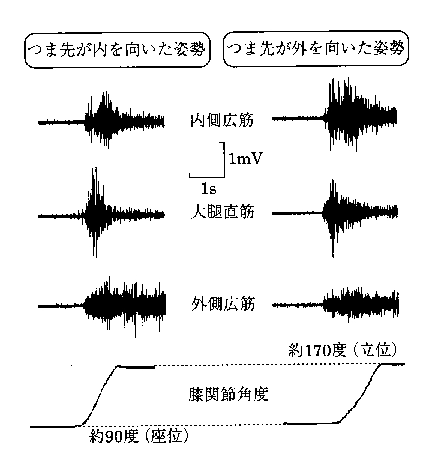
\includegraphics{emg003.eps}
   }
}
\caption{椅子から立ち上がり動作時における筋活動パターン.}
\label{fig:fig1}
\end{center}
\end{figure}

\subsection{正規化の方法を考えておく}

筋電図から筋活動のオン・オフや活動パターンを検討するだけなら,原波形そのままを用いてよい.
しかし,異なる被験者,異なる筋,異なる電極で計測した場合,筋活動量の計算値を個人間・筋間で直接比較するときには正規化が必要になる.
正規化の方法にはそれぞれ長所と短所があるため,目的によって正規化法を選ばないといけない.

\begin{itemize}
\item 100\%MVC法

ある動作局面の筋活動量を対象となる筋の最大随意収縮 (Maximal Voluntary Contraction: MVC)時の筋活動量に対する割合で表す方法.

\item 最大M波法

心理的限界の問題を払拭するために用いられる方法で,最大上の電気刺激を対象となる筋の神経束に与え,それによって現れる誘発筋電位反応 (これを最大M波)の振幅を基準値とする方法である.

\item 課題間比較法

2つの動作AとBを比較するとき,動作Aのときの筋活動量を動作Bのときの筋活動量に対する割合で示す方法.
\end{itemize}

\subsection{同期させる力学的信号を考えておく}

動作時の筋負担や動作特性などの計測・評価のために筋電位を記録する際は,動作との整合性を保ため,力学的信号(動作の情報)を同期させて記録しておく必要がある (例:図\ref{fig:fig1}).

\subsection{電気力学的遅延 (ElectroMechanical Delay: EMD):約30〜100 ms}

\begin{enumerate}
\item 筋収縮の開始
\item 緊張力の発生
\item 自重や初期張力に勝って張力信号や角度信号が変化しだす,あるいは筋放電が停止して張力信号や角度信号の変化も収束する
\end{enumerate}

一般的に,EMDは小筋群では短く,下肢などの大筋群では長い.
また,筋収縮速度,運動制御能力などによっても異なる.

\begin{equation}
M-RT = EMG-RT + EMD
\end{equation}
ここで,M-RTは機械的反応時間 (Mechanical Reaction Time: M-RT),EMG-RTは筋電図反応時間 (EMG-RT)を示す.
EMG-RTはPreMotor Time (PMT),EMDはMotor Time (MT)とも呼ばれている.

\begin{figure}
\begin{center}
\rotatebox{0}
{
   \scalebox{0.8}
   {
      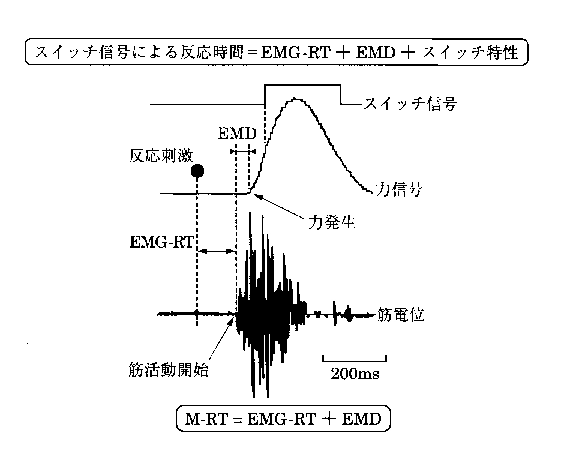
\includegraphics{emg004.eps}
   }
}
\caption{椅子から立ち上がり動作時における筋活動パターン.}
\label{fig:fig4}
\end{center}
\end{figure}

%\begin{figure}
%\begin{center}
%\rotatebox{0}
%{
%   \scalebox{0.8}
%   {
%      \includegraphics{imgs/img2.eps}
%   }
%}
%\caption{筋出力と筋活動量の相対的イメージ}
%\label{fig:fig2}
%\end{center}
%\end{figure}


\section{記録方法の選定と設定}

まず筋電図をどのように役立てるのかを考える必要がある.
\begin{itemize}
\item 筋放電開始,持続,停止をみて,動作に関与する筋が活動しているか否か (オン・オフ)や各筋の活動順序などの筋放電パターンを検討する.
\item どの程度使われているかなどの定量的解析をする
\item 筋電図の周波数解析を行う
\end{itemize}
目的によって,用いる電極の種類が異なるだけでなく,増幅器の設定もさまざまである.

\subsection{電極の種類 (図\ref{fig:fig6})}

\begin{figure}
\begin{center}
\rotatebox{0}
{
   \scalebox{0.8}
   {
      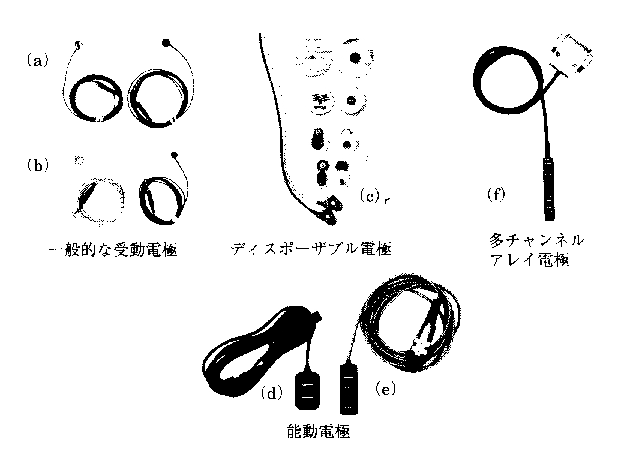
\includegraphics{emg005.eps}
   }
}
\caption{電極の種類}
\label{fig:fig6}
\end{center}
\end{figure}



\begin{itemize}
{\footnotesize
\item 受動電極 - 一般的に仕様される

	\begin{itemize}
	\item 電極と皮膚表面間の接触インピーダンスを下げるために、貼付部位に注意し、電極ペーストを使う必要がある
	\item 高インピーダンスのままでは温度、湿度、動きの影響を受けて
          分極電圧が変化し、ダイナミックな運動時に電極と皮膚表面との間
          を密接に接触できないためにアーチファクト(artifact, 人工的に発生する雑音)が発生する
	\end{itemize}
}
\item *能動電極 - 電極側で皮膚に近い高インピーダンスを電気的に作りだして、アーチファクトの発生を防ぐ仕様
	
	\begin{itemize}
	\item 電極ごとにバッファアンプ(ハイ・インピーダンスをロー・インピーダンスに変化させる)を内蔵
	\item 使用するときは、皮膚表面をかるくアルコールで拭き取るだけで、ダイナミックな運動であっても電極コードの揺れによるアーチファクトが発生しにくい計測が可能
	\item  能動電極 金属バーが10mm間隔で並んでいるものが多い。能動電極はアンプ部分を含め商品化が進み、小型計量化を中心にまだまだ進化している。
	\end{itemize}

\item 多チャンネルアレイ電極 -筋電位の伝搬パターンを探ることができる
\end{itemize}

\subsection{電極の特徴}

\begin{itemize}
\item 電極直径や電極間距離が長い場合

	\begin{itemize}
	\item メリット

		\begin{itemize}
		\item 対象となる筋全体的な筋活動を導出できる
		\item 筋繊維方向に対する電極のわずかなズレの影響を抑えられる
		\end{itemize}

	\item デメリット

		\begin{itemize}
		\item 高い周波数帯域の筋電を記憶しづらくなり、筋電位波形が平坦化する
		\item 隣接する筋からのクロストークが混入する可能性が高くなる
		\end{itemize}


	\end{itemize}

\item 電極直径が小さすぎる場合

	\begin{itemize}
	\item 皮膚と電極との接触インピーダンス(接触抵抗)が増え、ノイズを多く含んだ波形になる
	\item 電極間距離が短すぎると発汗によって2極が短絡(ショート)してしまう
	\end{itemize}
\end{itemize}

{\footnotesize
\subsection{推奨される電極の仕様}

\begin{itemize}

\item 受動電極の場合

\begin{itemize}
\item 露出金属部が直径5-10mm
\item 電極中心間距離10-20mm
\item 下肢などの大筋群から筋電位を導出する際は、直径・間隔ともに大きい電極でよい
\item 手指などの小筋群から導出する際は小さな電極を用いる方がよい

\end{itemize}

\end{itemize}
}

\subsection{増幅器の感度}

増幅器は表面筋電位の特性を考慮して設定しなければならない

\begin{itemize}
\item 感度(ゲイン)
	筋内で発生した電位は体表に到達するまでに1/1000以下に減衰する(体表で得られる電位の大きさ:数十マイクロV〜数mV).
	これを100〜10,000倍に増幅し、通常オシロスコープやペンレコーダなどの記録器上で1mV/cm程度になるように、感度を調整する.
\item 時定数
\item フィルタ
\end{itemize}

計測を始める前には、校正(calibration:CAL)スイッチを操作して、{\bf 校正値を記録しておくこと}を忘れてはならない.
校正値がないと,筋電位振幅の絶対値を計算したり,比較したりすることができなくなる.

\subsection{周波数特性}

\begin{itemize}
\item 帯域通過の下限周波数は時定数で表されることが多い(遮断周波数fc=1/(2πτ))
\item 表面筋電図の周波数成分は5〜500Hzに分布するといわれることから、標準的には0.03sを用いる(0.03sのとき5.3Hz以下がカットされる)
\item ローパスフィルタ(広域遮断フィルタ、ハイカット):標準1kHz以上が良い
\item ナイキストの定理より、サンプリングする観測信号の最高周波数成分がサンプリング周波数の半分以下でなければならない(表面筋電図の場合、その周波数成分は5Hzから500Hzまでといわれているので,広域遮断1kHz、サンプリング周波数2kHzがよく用いられている)
\end{itemize}

\subsection{入力インピーダンス}

増幅器の選定において、入力インピーダンス(増幅器の入力側に電圧を加えたときに、どれだけ電流が流れるかの比率.単位はM$\Omega$,$pF$)も重要である.
筋活動を正しく取り出すには増幅器の入力インピーダンスはできるだけ大きい
方がよい(一般的な入力インピーダンスの抵抗成分は10〜100M$\Omega$程度の
ものが多い.本研究室の仕様は200M$\Omega$.
わからない場合,メーカーに確認する方がよい.

\subsection{同相除去比 (Common Mode Rejection Ratio)}

増幅器の特性を表す指標の1つ.
弁別比ともいう.
CMRR が大きければ大きいほど性能のよい増幅器(オペアンプ)である.
同相除去比は増幅器に固有の特性で,装置を購入してしまったら変更したり設定できるものではないので購入前に確かめておくとよい.

\subsection{記録器}

筋電位記録中は,どのようなアーチファクトがどのようなタイミングで混入するか予測できないため,常に原波形をモニターし,導出されている筋電位波形が解析に耐えられるものかを調べておく.
つまり
\begin{itemize}
\item シグナル対ノイズ比(signal to noise ratio:S/N比)は十分か
\item 高い筋電位が出現したときに振り切れないか
\end{itemize}
などをチェックしておく.

\subsection{サンプリングレート}

\begin{itemize}
\item ビデオ画像:30-60Hz
\item 高速度カメラ:200Hz
\item 筋電位:1000Hz以上が望ましい(振幅情報の定量的評価を行う場合:できれば2kHz以上,少なくとも1kHz以上で行う.周波数解析の場合:5-10kHz,少なくとも2kHz.関与する筋のオン・オフ(活動しているか否か)だけをモニターし,力学的信号の検討を主に行う場合には,
あまり勧められないが,
力学的信号を記録する際の500Hz以下で筋電位信号もAD変換してしまう前例もある)
\end{itemize}

\subsection{購入した電極の情報}

\begin{itemize}
\item アクティブ電極 (能動電極)
\item チャンネル数 2
\item 電極間隔 12mm
\item 入力インピーダンス 200MΩ以上
\item 時定数 0.03 s
\item 弁別比(同相除去比) 110dB以上
\item 周波数特性 5-500Hz(-3dB)
\item 耐分極電圧 $\pm$600mV以上
\item 計測範囲 +6.25mV
\item 校正 登録方式*(校正表添付)
\item ケーブル長 130cm
\item 外形寸法 D12×H7×W23mm
\item 質量 約3g×2
\end{itemize}


\section{電極の貼付}
電極を貼付する下準備
\begin{itemize}
\item 神経筋接合部の位置と筋繊維の走行方向の確認
\item 皮膚抵抗を低減させる処理
\item アース電極を貼付する位置決め
\end{itemize}
\subsection{神経支配体を探す}
これまで電極貼付位置は,筋腹,あるいは{\bf 運動点}({\bf モーターポイント}:
一定強度の経皮的電気刺激によって最大の筋収縮が得られる点)としている場合が多い.
しかし,運動点は神経支配体(神経終末が筋に付着している部分)にあたり,筋
腹付近に分布している.仮りに,神経筋接合部を挟んで等距離に2つの電極を
貼付してしまうと,図\ref{fig:2-9}に示したように,接合部から両側(近位
と遠位)へ筋内伝播する電位がお互いを相殺して記録され,平坦な波形になっ
てしまう.したがって,筋腹付近で2つの電極で神経筋接合部を挟まないよう
に貼付するよう注意しなければならない。
とはいっても,神経支配帯は視認できないし,多チャンネルアレイ電極や電気
刺激を用いて神経接合部や運動点を同定するのは難しく,テクニックを要する.

そこで,筋腹付近をやや外して思い切って電極を貼ってしまう.ただし,その
まま計測を始めず,図\ref{fig:2-10}に示すように安静レベルの振幅と最大
筋出力時の振幅差が十分にあり,筋出力の増加とともに筋電位振幅も増大して
いるかを確かめておくことが重要である.2極が一体化された能動電極を用い
る場合でも,この作業は同様である.

さまざまな筋における神経支配帯の位置は''表面筋電図''の本のp146-p157が
参考になるが,個人差があることに注意.
%--図. -------------------------------
\begin{figure}[h]
  \centering
  \resizebox{6cm}{!}{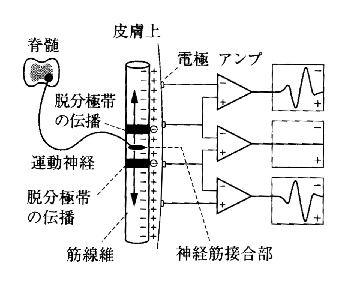
\includegraphics{emg006.eps}}
  \caption{神経筋接合部と電極との位置関係による筋電位波形の違い\label{fig:2-9}}
 \end{figure}
%----------------------------------
%--図. -------------------------------
\begin{figure}[h]
  \centering
  \resizebox{6cm}{!}{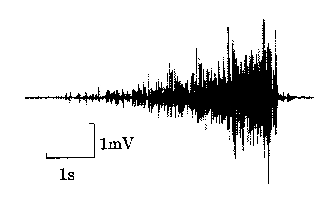
\includegraphics{emg007.eps}}
  \caption{良好な筋電図の例(筋出力の増大に伴う筋電位振幅の増大)\label{fig:2-10}}
 \end{figure}
%----------------------------------

\subsection{筋腹と筋繊維方向を確認する}
筋繊維の長軸ラインと2つの電極のラインがずれる(角度がつく)と筋電位波形
も歪んでしまうため,
\begin{itemize}
\item 筋の起始と停止(筋と骨の付着部分)
\item 紡錘筋であるか羽状筋であるかなどの筋の形状を解剖学の成書で調べておく.

紡錘筋(筋の基本形状.中央が膨らみ,両端が細い.)と羽状筋(筋中央(腱膜)
に向かって,筋繊維が斜めに集まる鳥の羽のような筋.)は筋肉における筋束の配置から分類されている.

\item 被験者に筋を収縮したり弛緩したりを繰り返してもらい,その筋の幅
  (端)を手で触りながら中央部を確認
\item 筋幅の中央部で,収縮させた際に筋が最も盛り上がる付近に目印をつけ
  る
\item 筋繊維方向に沿って,その目印を挟んだところに電極をおく(図
  \ref{fig:2-11})
\end{itemize}

関節角度の変化を伴う動的収縮の際には,筋収縮により皮膚上の電極位
置と神経支配帯の位置とが相対的にずれることによって影響がでる.周波数解
析をする場合には特に考慮しなければならない.対処法については以下の''ダ
イナミックな運動時での計測''を参考に. 

%--図. -------------------------------
\begin{figure}[h]
  \centering
  \resizebox{6cm}{!}{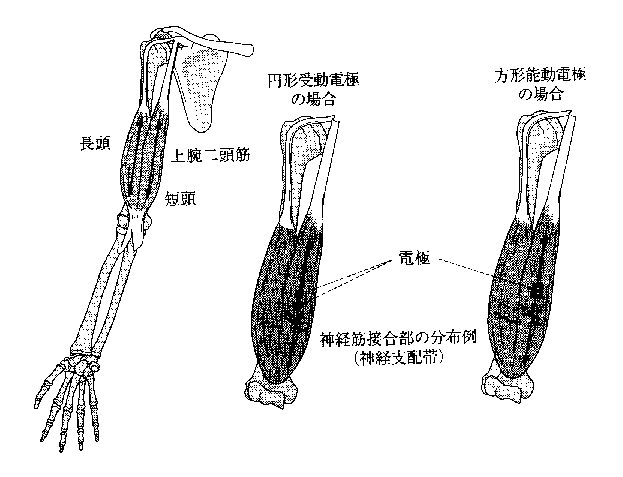
\includegraphics{emg008.eps}}
  \caption{上腕二頭筋における筋繊維走行および神経筋接合部の分布例と電
    極貼付例\label{fig:2-11}}
 \end{figure}
%----------------------------------

\subsection{ダイナミックな運動時での計測}
ダイナミックな運動時の表面筋電図計測における注意点.
\begin{itemize}
\item アーチファクトの混入と活動している筋線維に対する表面電極の位置.

→ 多チャンネル能動アレイ表面電極を計測や解析に利用.
\item 双極差動導出に与える神経支配帯の影響.

神経支配帯(神経筋接合部が狭い範囲に集中している部位)を避けて電極を貼付する事が理想だが,どの時点でどの神経支配帯
が影響を与えているかは計測してみないと分からない.
また,筋のサイズや解剖学的な理由で神経支配帯の影響をどうしても避けられ
ない場面がある.

→ 多チャンネルアレイ電極を使い,神経支配帯の影響を受けていないいずれ
かの双極差動導出ペアを選択する方法が提案されている.
\end{itemize}

各双極差動導出ペアから推定されたチャンネル$i$の{\bf 積分筋電図}(Integrated
EMG : $IEMG_i(t)$),表面筋電図の{\bf 平均周波数}(MeaN Power Frequency :
$MNF_i(t)$)に対して
\begin{align}
  IEMG_c(t)=max_i\{IEMG_i(t)\} \\
  MNF_c(t)=min_i\{MNF_i(t)\}
\end{align}
のように比較することで,神経支配帯の影響を抑えた$IEMG_c(t)$と
$MNF_c(t)$が得られる.


\subsection{皮膚抵抗を低減する}
皮膚抵抗の低減には,昔は紙ヤスリなどで擦っていたが,皮膚へのダメージも
あるので,現在ではほとんど行わない.

{\footnotesize
受動電極を用いる場合
\begin{itemize}
\item コンパウンドを混ぜたペーストがあるので,それを脱脂綿などにつけて
  擦り,アルコールで拭く
\item さらに乾いた脱脂綿などで乾かすなどを十分してから電極を貼付
\item それでも基線の揺れやノイズが発生する場合には{\bf プリパレーショ
    ン}(針の先で電極中央部にあたる皮膚の表組織1枚を剥す
作業)を行なう
\end{itemize}
}

*能動電極を用いる場合
\begin{itemize}
\item アルコールで拭く(多分この作業のみで十分)
\item 皮膚処理用のペーストなどで擦る
\end{itemize}

\subsection{電極を固定する}
ディスポータブルタイプ以外の受動電極
\begin{itemize}
\item カップの中に{\bf 電極ペースト}(高い導電性を持つ糊状のもの)を注入する

ペーストは表面張力が効いている状態のように,カップからペーストが微妙に
盛り上がっている程度がちょうど良い.
\item 電極を貼付位置に置き,テープなどで皮膚に固定する

テープはサージカルテープなど,粘着力が強くて薄いものが良い.専用の両面
固定シールを使うと便利.
\item ペーストが皮膚になじむ(接触インピーダンスが落ち着く)まで待つ(貼
  付後10〜15分)

なじむ前に計測を始めると,最初と筋電図はノイズ成分が残り,基線が太くな
る場合がある(図\ref{fig:2-12}).

\item 確認作業として電極間抵抗(電極間インピーダンス)を測定しておく

一般に20k$\Omega$以下で,できれば5k$\Omega$以下であることが望ましい.
\end{itemize}
%--図. -------------------------------
\begin{figure}[h]
  \centering
  \resizebox{6cm}{!}{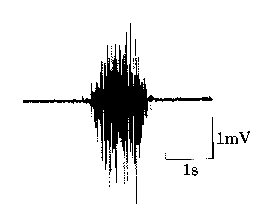
\includegraphics{emg009.eps}}
  \caption{受動電極貼付直後の筋電図の例(基線が比較的太い)\label{fig:2-12}}
 \end{figure}
%----------------------------------

\subsection{アース電極を貼る}
\begin{itemize}
\item {\bf 導出電極}(記録電極,信号電極,探査電極)

筋電位を導出する筋の直上に貼付する電極

\item {\bf アース電極}({\bf 接地電極})

筋電位を導出する筋とは無関係の部位に貼付する電極
\end{itemize}

アース電極にもさまざまな種類があるが,導出電極を貼付する場合と同じく皮
膚抵抗を低減させる処置をしっかりと施しておかなければならない.

アース電極貼付位置
\begin{itemize}
\item 皮膚直下に筋がない

手首,足首,肘部,膝蓋骨上,第7頸椎付近
\item 筋から遠い部位
\end{itemize}

アース電極を1つ貼付してもノイズが十分に除去できないときは,面積の大き
いアース電極を用いたり,複数個貼付する.
裸足になって接地コネクタに接続された大きな導電板の上で動作することも一
案.ただし,アース電極を複数個用いる際は,機器側の同一アース端子に接続
する.


\section{諸問題対策}
\subsection{振幅が小さい}
電極の位置を変えてみると解決する場合が多い.
\begin{itemize}
\item 電極間が広すぎる
\item 2つの電極のラインが筋繊維方向とずれている
\item たまたま神経筋接合部の直上付近に電極を貼ってしまった
\end{itemize}
などが原因となっている場合が多い

\subsection{交流雑音を除く}
{\bf 交流雑音}({\bf ハム})が見られる場合は,最初にアース電極の接続を再
確認する.アース電
極のリード線は通常,計測機器のアース・コネクタに繋がり,最終的には実験
室の壁などにある接地コネクタに接続される.これらの各接続部が確実に固定
されているか確認する.

それでもノイズ成分が残る場合には以下を参考に,ありとあらゆる方策を実行す
る.
\begin{enumerate}
\item 皮膚に添付するアース電極の接触面積を増やす
\item 電極からのリード線おのおのがシールドされているタイプのものを用い
  る
\item 計測時に使用する椅子,机,ベットなどの金属部分を接地コネクタにつ
  なぐ
\item 周辺にある計測には関係ないすべての電源機器をOFFにする
\item 関係のない電気機器の電源コードも抜いておく
\item 磁界が生ずる可能性があるので電源コードをグルグルまるめたりしない
\item 蛍光灯もOFFにしてみる
\item 電源コードを繋いだ同じコンセント(分岐器など)から,他の機器類が発
生するノイズは拾っている場合もあるので,筋電位計測関係の機器と他の機器
のコンセントを別系統にしてみる
\item 運動付加装置のモーターなどがノイズ源で,OFFできず困る場合は,少
  しでもそれを遠ざける,あるいは小型シールド箱にいれてしまう
\end{enumerate}

交流雑音が混入した筋電図の例は図\ref{fig:2-13}. 
交流雑音の除去には{\bf ハム・フィルタ}(50Hzあるいは60Hz付近を選択的
に減衰させる)も有効であるが,筋電位成分にも影響を与えてしまうため,で
きるだけ用いず最終手段とした方がよい.

%--図. -------------------------------
\begin{figure}[h]
  \centering
  \resizebox{6cm}{!}{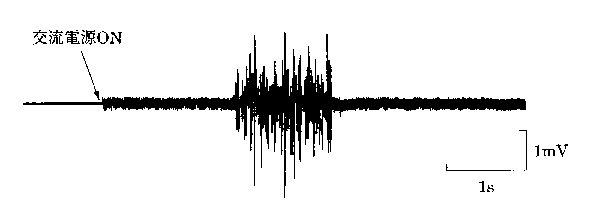
\includegraphics{emg010.eps}}
  \caption{交流雑音の入った筋電図の例\label{fig:2-13}}
 \end{figure}
%----------------------------------

\subsection{接地コネクタを疑う}
壁や床に埋め込まれている接地コネクタが,隣や上下階など他の実験室と共用
(同系統)である場合,他の実験室にある機器から発生するノイズを逆にもらっ
てしまう事もある.別系統の接地コネクタを利用するか,市販のアース棒を購
入し,実験室近くの地面に穴を掘って埋め,それを用いると効果がある時もあ
る.
ただし,可能なかぎり筋電位の導出に関係するアースは1つに統合した方がよ
い.

\subsection{基線が揺れる}
電極リード線が動作に伴って揺れる,あるいは引っ張られることにより,モー
ション・アーチファクトが混入し,筋電位の{\bf 基線}が揺れる場合がある
(図\ref{fig:2-14}).まずは関節可動域を妨げないように注意しながら,サー
ジカルテープなどでリード線を皮膚の上にとめるとよい.また,この主のノイ
ズの周波数は比較的低いので,10〜20Hz以下をカットすれば,主な筋電位成分
を損なうことなく基線の揺れを除くことができる.

%--図. -------------------------------
\begin{figure}[h]
  \centering
  \resizebox{6cm}{!}{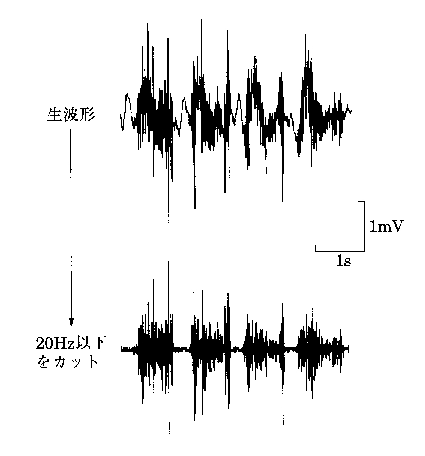
\includegraphics{emg011.eps}}
  \caption{モーション・アーチファクト入りの筋電図の例(基線の揺れ)
    \label{fig:2-14}}
 \end{figure}
%----------------------------------

すばやく大きな動作中における筋電図は,20Hz以下ではカットできないモーショ
ン・アーチファクトが残ることがある.この場合,フィルタの設定を変えるか,
次定数を0.03sから0.003sに変える方法がある.しかし,次定数0.003sを用い
ると53.1Hz以下がカットされることになるので,筋電位の低周波成分の一部も
損なわれる問題がある.プリパレーションによって皮膚抵抗を下げたり,能動
電極を用いることで基線揺れを抑えられる.

大胸筋や僧帽筋など体幹の筋から筋電位を導出すると,規則的に基線が揺れる
場合がある.大体0.8秒から1秒に1回のペースで現れているのなら,心電位で
ある.導出電極とアース電極で心臓を挟まないように,アース電極の位置を変
えれば消える場合が多い.

\end{document}
